\documentclass{article}

% Recommended, but optional, packages for figures and better typesetting:
\usepackage{microtype}
\usepackage{graphicx}
\usepackage{subfigure}
\usepackage{booktabs} % for professional tables

\usepackage{mathtools}
\usepackage{physics}

% hyperref makes hyperlinks in the resulting PDF.
% If your build breaks (sometimes temporarily if a hyperlink spans a page)
% please comment out the following usepackage line and replace
% \usepackage{icml2020} with \usepackage[nohyperref]{icml2020} above.
\usepackage{hyperref}

% Attempt to make hyperref and algorithmic work together better:
\newcommand{\theHalgorithm}{\arabic{algorithm}}

% Use the following line for the initial blind version submitted for review:
% \usepackage{icml2020}

% If accepted, instead use the following line for the camera-ready submission:
\usepackage[accepted]{icml2020}

% The \icmltitle you define below is probably too long as a header.
% Therefore, a short form for the running title is supplied here:
\icmltitlerunning{Optimal flocking with a genetic algorithm}

\begin{document}

\twocolumn[
\icmltitle{Optimal boid flocking with a genetic algorithm}

% It is OKAY to include author information, even for blind
% submissions: the style file will automatically remove it for you
% unless you've provided the [accepted] option to the icml2020
% package.

% List of affiliations: The first argument should be a (short)
% identifier you will use later to specify author affiliations
% Academic affiliations should list Department, University, City, Region, Country
% Industry affiliations should list Company, City, Region, Country

% You can specify symbols, otherwise they are numbered in order.
% Ideally, you should not use this facility. Affiliations will be numbered
% in order of appearance and this is the preferred way.
% \icmlsetsymbol{equal}{*}

\begin{icmlauthorlist}
\icmlauthor{Frederik J. Mellbye}{to}
\end{icmlauthorlist}

\icmlaffiliation{to}{Institute for Computational and Mathematical Engineering, Stanford University, Stanford, USA}

\icmlcorrespondingauthor{Frederik J. Mellbye}{frederme@stanford.edu}

% You may provide any keywords that you
% find helpful for describing your paper; these are used to populate
% the "keywords" metadata in the PDF but will not be shown in the document
\icmlkeywords{Machine Learning, ICML}

\vskip 0.3in
]

% this must go after the closing bracket ] following \twocolumn[ ...

% This command actually creates the footnote in the first column
% listing the affiliations and the copyright notice.
% The command takes one argument, which is text to display at the start of the footnote.
% The \icmlEqualContribution command is standard text for equal contribution.
% Remove it (just {}) if you do not need this facility.

\printAffiliationsAndNotice{}  % leave blank if no need to mention equal contribution
% \printAffiliationsAndNotice{\icmlEqualContribution} % otherwise use the standard text.

\begin{abstract}
A genetic evolution-based approach is used to determine the coefficients of a boids model for optimal flocking. The model is inspired by the original Reynolds model, and adds predators. The results show that ...
\end{abstract}

\section{Introduction}
\label{sec:introduction}
Boids, developed by Craig Reynolds in 1986 \cite{reynolds:1987:CG}, is an artificial life program that simulates flocking, herding and schooling behavour typically seen in animals in nature. The behavior of boids is governed by a set of simple rules, based on the proximity and heading of other nearby individuals.

Versions of the boids framework have been used in various applications, e.g. to generate realistic-looking flocks of flying animals and schooling fish. Examples are birds in the 1998 video game \textit{Half-Life}, and bat swarms in the 1992 feature film \textit{Batman Returns}. Versions of the boids framework have also been used in swarm robotics, for which flocking behaviour is often desired \cite{swarm}. In biology, the boids model has been important in understanding how schools of fish form and behave because of their close similarities \cite{reynolds:1987:CG}.

Short explanation of the boids system - 2D grid, random init.

Finding a good set of parameter values for boids is therefore of interest.
This project adds predators that attack prey boids, with the notion of group defense - sufficiently large groups of prey boids are able to fend off attacking predators. A genetic algorithm is used to discover coeffient values that tend to survive the boid simulations.

\section{Background}
\label{sec:background}
Boid implementations commonly use a heuristic technique to determine the coefficients, through visualizations of the boid system. The coefficients were chosen for different behaviors, such as matching behaviour seen in nature for movies \cite{reynolds:1987:CG}.

Optimization approaches have also been used. Different approaches include maximizing the total aligntment or minimizing the avarage distance between boids. Particle swarm and genetic optimization techniques have been applied to optimize for this behavior \cite{ntnu}.

This project:
Objective -> Maximize number of survivors. Randomness in init -> randomness in objective. Overarching goal: optimize flocking. So different approach.

\section{Approach}
\label{sec:approach}
\subsection{Boids system}
\subsubsection{Steering forces}
\begin{figure*}
  \centering
  \includegraphics[width=.25\linewidth]{images/separation.png}
  \includegraphics[width=.25\linewidth]{images/alignment.png}
  \includegraphics[width=.25\linewidth]{images/cohesion.png}
  \caption{Steering forces on prey boids. From the left: Separation, alignment and cohesion \cite{reynolds:1987:CG}.}
  \label{fig:preyforces}
\end{figure*}

Prey boids have the three original steering forces; cohesion, separation and alignment \cite{reynolds:1987:CG}. These are depicted in Figure~\ref{fig:preyforces}.

The cohesion force $F_c$ on boid $b_j$ is given by
\begin{align}
  F_c = c_c \frac{1}{n-1} \sum_{i \neq j}^{n} x_i - x_j
\end{align}
where $c_c$ is a corresponding coefficient on the force, and $x_i$ is the position of $b_i$. It draws boids closer to the general position of neighboring boids.

Similarly, the separation force is given by
\begin{align}
  F_s = c_s \frac{1}{n-1} \sum_{i \neq j}^{n} \frac{x_i - x_j}{\norm{x_i - x_j}_2}
\end{align}
This force only considers boids that are very close, and ensures boids do not fly too close to each other. In some sense this simulates that the boids have some size and avoid crashing.

Finally, the alignment force is
\begin{align}
  F_a = c_a \frac{1}{n-1} \sum_{i \neq j}^{n} v_i - v_j
\end{align}
where $v_i$ is the velocity vector of $b_i$. Boids steer towards the average heading of neighboring boids.

The forces are combined to produce a total force, which is clipped, simulating how animals only can turn at certain rates. The total force is therefore given by
\begin{align*}
  F = \max(F_c + F_s + F_a, F_\text{max})
\end{align*}
The boid masses are normalized, so the force is the acceleration. We also have a time step $\Delta t = 1$. Therefore, the velocity and position updates are
\begin{align*}
  v^{(k+1)} &= v^{(k)} + F \\
  x^{(k+1)} &= x^{(k)} + \frac{v^{(k+1)}}{\norm{v^{(k+1)}}_2}
\end{align*}
Note that the velocity is normalized. This paper assumes that all boids fly at their max speed $v_\text{max}$ at all times.

Predators follow three forces; they hunt the nearest prey boid, flee from prey boids if too many prey boids are present (simulating how prey animals often are able to fend of predators when grouped together) and separation. These added forces are depicted in Figure~\ref{fig:predatorforces}.

\begin{figure*}
  \centering
  \includegraphics[width=.25\linewidth]{images/chase.png}
  \includegraphics[width=.25\linewidth]{images/avoid.png}
  \caption{Hunt and flee steering forces on predator boids. Modified versions of images from \cite{reynolds:1987:CG}.}
  \label{fig:predatorforces}
\end{figure*}

\subsubsection{Initialization}
In each simulation, the boids $b_i$ have randomly initialized positions and velocities. Let $w$ and $h$ denote the system width and height respectively. The positions are sampled uniformly, i.e.
\begin{align*}
  x_i \sim \begin{bmatrix} u(0.2w, 0.5w) \\ u(0.2h, 0.8h) \end{bmatrix}
\end{align*}
where $u(a,b)$ denotes a uniform random variable on $[a,b]$. This way prey boids spawn on the left half of the environment. Predators similarly spawn on the other half. This attempts to ensure that prey boids are not killed immediately before they have the chance to flock.

The velocities are set to
\begin{align*}
  v_i \sim \begin{bmatrix} 1 \\ u(0,1) \end{bmatrix}
\end{align*}
i.e. towards the center with some random $y$-component.

\subsection{Genetic algorithm}
The goal of this project is to determine the set of coefficients of an entire flock of prey boids that maximizes their survival in the presence of predators. The design is the set of coefficients of all boids $\{c_i\}_{i=1}^{n}$. A genetic algorithm is employed to optimize these coefficients for flocking, which leads to survival.

Genetic algorithm approaches commonly have three components; selection, crossover and mutation \cite{kochenderfer}. The fashion in which these are performed commonly differs based on the particular application and the way the chromosomes are encoded.

\subsubsection{Selection}
In each simulation, a subset of the prey boids survive through the simulation. In this project, the selection step simply selects the survivors of each generation. This is motivated from the principle of natural selection.

\subsubsection{Crossover}
Crossover is performed as follows: For each new boid, for each coefficient,
the new boid gets one of the parents values with uniform probability. This way, traits that predict survival are propagated from one generation to the next.

\subsubsection{Mutation}
To introduce the possibility of new variations, mutations are sporadically added in the form of gaussian noise. With probability $0.1$, we add $\mathcal{N}(0, \sigma^2)$ noise to a particular coefficient of a new boid. The variance is tuned such that a shift in coefficient values is seen over many generations.

\begin{table*}
  \centering
  \caption{Parameters used for the genetic algorithm and boids simulation. Most of these were tuned heuristically as the system was developed.}
  \label{tbl:params}
\begin{tabular}{*4l} \toprule
\emph{Name}       & \emph{Symbol} & \emph{Value} & \emph{Description} \\ \midrule
Mutation probability& & 0.1 & Probability of mutation for a particular coefficient \\
Mutation spread        &  $\sigma$      & 0.1  & Standard deviation of the mutation   \\
Separation range           &        &  &     \\
Prey force ranges         &        &  2000 &\\
Kill range          &        & 4.0     & \\
Hunting coefficient & $c_h$ &       &\\
Flee distance & & 80     \\
Predator $v_\text{max}$ &       & 1.1     & \\
Prey $v_\text{max}$ &        & 1.0     & \\
Predator max force & $F_\text{max, predator}$ & 0.1& \\
Prey max force & $F_\text{max, prey}$ & 0.04 &\\\bottomrule
\end{tabular}
\end{table*}

\subsection{Computational considerations}
For performance reasons, the implementation of the boids framework and genetric algorithm was done in C++.

With a naive implementation the computation of the steering forces is $\mathcal{O}(n^2)$. For each boid, the positions of all other boids are required. This is clearly not feasible for simulations with many boids and many generations of evolution.

To reduce the computational load, each boid locally keeps track of it's nearest neighbors and only use these to compute steering. This allows constant time lookup of neighbors, which greatly simplifies the complexity, at the cost of the small error introduced by the approximation. The list of neighbors is updated with a particular frequency, for this project every 10 time steps.

\section{Results}
\label{sec:results}
Figures~\ref{fig:survival} and~\ref{fig:coeffs} show the number of survivors and coefficient statistics over the course of 300 generations of evolution.

\begin{figure}
  \centering
  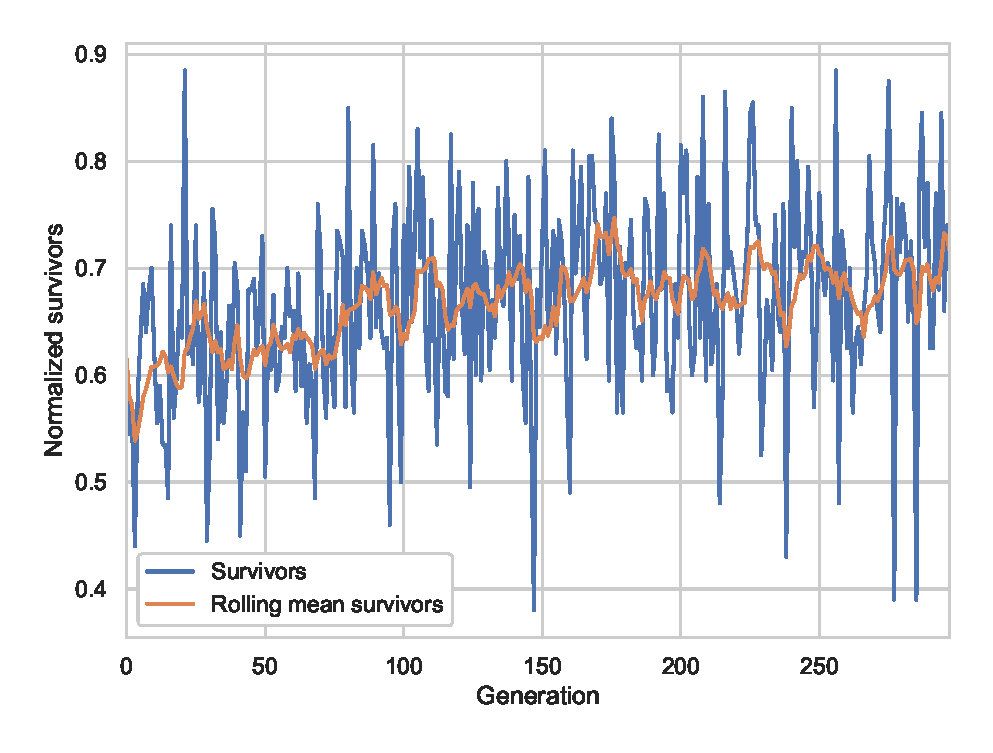
\includegraphics[width=\linewidth]{figures/survival.eps}
  \caption{Proportion of boids that survive each generation. The orange line shows the mean of the last 10 numbers of survivors. It is clear that there is high randomness in the simulations, likely due to the inherent randomness of each simulation. A lot of boids do not have time to move towards other flockmates before a predator reaches them.}
  \label{fig:survival}
\end{figure}

\begin{figure}
  \centering
  \includegraphics[width=\linewidth]{figures/coeffs.pdf}
  \caption{Mean coefficient value across all boids of each particular generation. The shaded regions show the standard deviations of the coefficients.}
  \label{fig:coeffs}
\end{figure}

\section{Conclusion}
\label{sec:conclusion}
Discuss how results are unreliable because of large degree of randomness.

\section{Future directions}
\label{sec:future}
Better objective function/algorithm.

More realistic physics simulation -> interesting applications. E.g. drone swarms. Applications in e.g. defense systems.

Also optimize predator behaviour (this could in turn further optimize prey behaviour. Turns into a min-max problem.)

Add obstacles and potentially add some goal area to get to.


% In the unusual situation where you want a paper to appear in the
% references without citing it in the main text, use \nocite

\bibliography{references}
\bibliographystyle{icml2020}

%%%%%%%%%%%%%%%%%%%%%%%%%%%%%%%%%%%%%%%%%%%%%%%%%%%%%%%%%%%%%%%%%%%%%%%%%%%%%%%
%%%%%%%%%%%%%%%%%%%%%%%%%%%%%%%%%%%%%%%%%%%%%%%%%%%%%%%%%%%%%%%%%%%%%%%%%%%%%%%


\end{document}


% This document was modified from the file originally made available by
% Pat Langley and Andrea Danyluk for ICML-2K. This version was created
% by Iain Murray in 2018, and modified by Alexandre Bouchard in
% 2019 and 2020. Previous contributors include Dan Roy, Lise Getoor and Tobias
% Scheffer, which was slightly modified from the 2010 version by
% Thorsten Joachims & Johannes Fuernkranz, slightly modified from the
% 2009 version by Kiri Wagstaff and Sam Roweis's 2008 version, which is
% slightly modified from Prasad Tadepalli's 2007 version which is a
% lightly changed version of the previous year's version by Andrew
% Moore, which was in turn edited from those of Kristian Kersting and
% Codrina Lauth. Alex Smola contributed to the algorithmic style files.
